\documentclass[10pt,compress,t,notes=noshow, xcolor=table]{beamer}
\newcommand{\btVFill}{\vskip0pt plus 1filll}
\newcommand\hmmax{0}
\newcommand\bmmax{0}
\usepackage[]{graphicx}
% graphicx is loaded via lmu-lecture.sty as well
\usepackage[]{color}
% maxwidth is the original width if it is less than linewidth
% otherwise use linewidth (to make sure the graphics do not exceed the margin)
\makeatletter
\def\maxwidth{ %
  \ifdim\Gin@nat@width>\linewidth
    \linewidth
  \else
    \Gin@nat@width
  \fi
}
\makeatother

% ---------------------------------%
% latex-math dependencies, do not remove:
% - mathtools
% - bm
% - siunitx
% - dsfont
% - xspace
% ---------------------------------%

%--------------------------------------------------------%
%       Language, encoding, typography
%--------------------------------------------------------%

\usepackage[english]{babel}
\usepackage[utf8]{inputenc} % Enables inputting UTF-8 symbols
% Standard AMS suite (loaded via lmu-lecture.sty)
\usepackage{amsmath,amsfonts,amssymb}

% Font for double-stroke / blackboard letters for sets of numbers (N, R, ...)
% Distribution name is "doublestroke"
% According to https://mirror.physik.tu-berlin.de/pub/CTAN/fonts/doublestroke/dsdoc.pdf
% the "bbm" package does a similar thing and may be superfluous.
% Required for latex-math
\usepackage{dsfont}

% bbm – "Blackboard-style" cm fonts (https://www.ctan.org/pkg/bbm)
% Used to be in common.tex, loaded directly after this file
% Maybe superfluous given dsfont is loaded
% TODO: Check if really unused?
% \usepackage{bbm}

% bm – Access bold symbols in maths mode - https://ctan.org/pkg/bm
% Required for latex-math, preferred over \boldsymbol
% https://tex.stackexchange.com/questions/3238/bm-package-versus-boldsymbol
\usepackage{bm}

% pifont – Access to PostScript standard Symbol and Dingbats fonts
% Used for \newcommand{\xmark}{\ding{55}, which is never used
% aside from lecture_advml/attic/xx-automl/slides.Rnw
% \usepackage{pifont}

% Quotes (inline and display), provdes \enquote
% https://ctan.org/pkg/csquotes
\usepackage{csquotes}

% Adds arg to enumerate env, technically superseded by enumitem according
% to https://ctan.org/pkg/enumerate
% Replace with https://ctan.org/pkg/enumitem ?
% Even better: enumitem is not really compatible with beamer and breaks all sorts of things
% particularly the enumerate environment. The enumerate package also just isn't required
% from what I can tell so... don't re-add it I guess?
% \usepackage{enumerate}

% Line spacing - provides \singlespacing \doublespacing \onehalfspacing
% https://ctan.org/pkg/setspace
% \usepackage{setspace}

% mathtools – Mathematical tools to use with amsmath
% https://ctan.org/pkg/mathtools?lang=en
% latex-math dependency according to latex-math repo
\usepackage{mathtools}

% Maybe not great to use this https://tex.stackexchange.com/a/197/19093
% Use align instead -- TODO: Global search & replace to check, eqnarray is used a lot
% $ rg -f -u "\begin{eqnarray" -l | grep -v attic | awk -F '/' '{print $1}' | sort | uniq -c
%   13 lecture_advml
%   14 lecture_i2ml
%    2 lecture_iml
%   27 lecture_optimization
%   45 lecture_sl
\usepackage{eqnarray}

% For shaded regions / boxes
% Used sometimes in optim
% https://www.ctan.org/pkg/framed
\usepackage{framed}

%--------------------------------------------------------%
%       Cite button (version 2024-05)
%--------------------------------------------------------%
% Note this requires biber to be in $PATH when running,
% telltale error in log would be e.g. Package biblatex Info: ... file 'authoryear.dbx' not found
% aside from obvious "biber: command not found" or similar.
% Tried moving this to lmu-lecture.sty but had issues I didn't quite understood,
% so it's here for now.

\usepackage{textcase} % for \NoCaseChange
\usepackage{hyperref}

% Only try adding a references file if it exists, otherwise
% this would compile error when references.bib is not found
\IfFileExists{references.bib} {
  \usepackage{usebib}
  \usepackage[backend=biber, style=authoryear]{biblatex}

  \addbibresource{./references.bib}
  \bibinput{references}
}

\newcommand{\citelink}[1]{%
\NoCaseChange{\resizebox{!}{9pt}{\protect\beamergotobutton{\href{\usebibentry{\NoCaseChange{#1}}{url}}{\begin{NoHyper}\cite{#1}\end{NoHyper}}}}}%
}

%--------------------------------------------------------%
%       Displaying code and algorithms
%--------------------------------------------------------%

% Reimplements verbatim environments: https://ctan.org/pkg/verbatim
% verbatim used sed at least once in
% supervised-classification/slides-classification-tasks.tex
% Removed since code should not be put on slides anyway
% \usepackage{verbatim}

% Both used together for algorithm typesetting, see also overleaf: https://www.overleaf.com/learn/latex/Algorithms
% algorithmic env is also used, but part of the bundle:
%   "algpseudocode is part of the algorithmicx bundle, it gives you an improved version of algorithmic besides providing some other features"
% According to https://tex.stackexchange.com/questions/229355/algorithm-algorithmic-algorithmicx-algorithm2e-algpseudocode-confused
\usepackage{algorithm}
\usepackage{algpseudocode}

%--------------------------------------------------------%
%       Tables
%--------------------------------------------------------%

% multi-row table cells: https://www.namsu.de/Extra/pakete/Multirow.html
% Provides \multirow
% Used e.g. in evaluation/slides-evaluation-measures-classification.tex
\usepackage{multirow}

% colortbl: https://ctan.org/pkg/colortbl
% "The package allows rows and columns to be coloured, and even individual cells." well.
% Provides \columncolor and \rowcolor
% \rowcolor is used multiple times, e.g. in knn/slides-knn.tex
\usepackage{colortbl}

% long/multi-page tables: https://texdoc.org/serve/longtable.pdf/0
% Not used in slides
% \usepackage{longtable}

% pretty table env: https://ctan.org/pkg/booktabs
% Is used
% Defines \toprule
\usepackage{booktabs}

%--------------------------------------------------------%
%       Figures: Creating, placing, verbing
%--------------------------------------------------------%

% wrapfig - Wrapping text around figures https://de.overleaf.com/learn/latex/Wrapping_text_around_figures
% Provides wrapfigure environment -used in lecture_optimization
\usepackage{wrapfig}

% Sub figures in figures and tables
% https://ctan.org/pkg/subfig -- supersedes subfigure package
% Provides \subfigure
% \subfigure not used in slides but slides-tuning-practical.pdf errors without this pkg, error due to \captionsetup undefined
\usepackage{subfig}

% Actually it's pronounced PGF https://en.wikibooks.org/wiki/LaTeX/PGF/TikZ
\usepackage{tikz}

% No idea what/why these settings are what they are but I assume they're there on purpose
\usetikzlibrary{shapes,arrows,automata,positioning,calc,chains,trees, shadows}
\tikzset{
  %Define standard arrow tip
  >=stealth',
  %Define style for boxes
  punkt/.style={
    rectangle,
    rounded corners,
    draw=black, very thick,
    text width=6.5em,
    minimum height=2em,
    text centered},
  % Define arrow style
  pil/.style={
    ->,
    thick,
    shorten <=2pt,
    shorten >=2pt,}
}

%--------------------------------------------------------%
%       Beamer setup and custom macros & environments
%--------------------------------------------------------%

% Main sty file for beamer setup (layout, style, lecture page numbering, etc.)
% For long-term maintenance, this may me refactored into a more modular set of .sty files
\usepackage{../../style/lmu-lecture}
% Custom itemize wrappers, itemizeS, itemizeL, etc
\usepackage{../../style/customitemize}
% Custom framei environment, uses custom itemize!
\usepackage{../../style/framei}
% Custom frame2 environment, allows specifying font size for all content
\usepackage{../../style/frame2}
% Column layout macros
\usepackage{../../style/splitV} 

% Used regularly
\let\code=\texttt

% Not sure what/why this does
\setkeys{Gin}{width=0.9\textwidth}

% -- knitr leftovers --
% Used often in conjunction with \definecolor{shadecolor}{rgb}{0.969, 0.969, 0.969}
% Removing definitions requires chaning _many many_ slides, which then need checking to see if output still ok
\definecolor{fgcolor}{rgb}{0.345, 0.345, 0.345}
\definecolor{shadecolor}{rgb}{0.969, 0.969, 0.969}
\newenvironment{knitrout}{}{} % an empty environment to be redefined in TeX

%-------------------------------------------------------------------------------------------------------%
%  Unused stuff that needs to go but is kept here currently juuuust in case it was important after all  %
%-------------------------------------------------------------------------------------------------------%

% \newcommand{\hlnum}[1]{\textcolor[rgb]{0.686,0.059,0.569}{#1}}%
% \newcommand{\hlstr}[1]{\textcolor[rgb]{0.192,0.494,0.8}{#1}}%
% \newcommand{\hlcom}[1]{\textcolor[rgb]{0.678,0.584,0.686}{\textit{#1}}}%
% \newcommand{\hlopt}[1]{\textcolor[rgb]{0,0,0}{#1}}%
% \newcommand{\hlstd}[1]{\textcolor[rgb]{0.345,0.345,0.345}{#1}}%
% \newcommand{\hlkwa}[1]{\textcolor[rgb]{0.161,0.373,0.58}{\textbf{#1}}}%
% \newcommand{\hlkwb}[1]{\textcolor[rgb]{0.69,0.353,0.396}{#1}}%
% \newcommand{\hlkwc}[1]{\textcolor[rgb]{0.333,0.667,0.333}{#1}}%
% \newcommand{\hlkwd}[1]{\textcolor[rgb]{0.737,0.353,0.396}{\textbf{#1}}}%
% \let\hlipl\hlkwb

% \makeatletter
% \newenvironment{kframe}{%
%  \def\at@end@of@kframe{}%
%  \ifinner\ifhmode%
%   \def\at@end@of@kframe{\end{minipage}}%
%   \begin{minipage}{\columnwidth}%
%  \fi\fi%
%  \def\FrameCommand##1{\hskip\@totalleftmargin \hskip-\fboxsep
%  \colorbox{shadecolor}{##1}\hskip-\fboxsep
%      % There is no \\@totalrightmargin, so:
%      \hskip-\linewidth \hskip-\@totalleftmargin \hskip\columnwidth}%
%  \MakeFramed {\advance\hsize-\width
%    \@totalleftmargin\z@ \linewidth\hsize
%    \@setminipage}}%
%  {\par\unskip\endMakeFramed%
%  \at@end@of@kframe}
% \makeatother

% \definecolor{shadecolor}{rgb}{.97, .97, .97}
% \definecolor{messagecolor}{rgb}{0, 0, 0}
% \definecolor{warningcolor}{rgb}{1, 0, 1}
% \definecolor{errorcolor}{rgb}{1, 0, 0}
% \newenvironment{knitrout}{}{} % an empty environment to be redefined in TeX

% \usepackage{alltt}
% \newcommand{\SweaveOpts}[1]{}  % do not interfere with LaTeX
% \newcommand{\SweaveInput}[1]{} % because they are not real TeX commands
% \newcommand{\Sexpr}[1]{}       % will only be parsed by R
% \newcommand{\xmark}{\ding{55}}%

% textpos – Place boxes at arbitrary positions on the LATEX page
% https://ctan.org/pkg/textpos
% Provides \begin{textblock}
% TODO: Check if really unused?
% \usepackage[absolute,overlay]{textpos}

% -----------------------%
% Likely knitr leftovers %
% -----------------------%

% psfrag – Replace strings in encapsulated PostScript figures
% https://www.overleaf.com/latex/examples/psfrag-example/tggxhgzwrzhn
% https://ftp.mpi-inf.mpg.de/pub/tex/mirror/ftp.dante.de/pub/tex/macros/latex/contrib/psfrag/pfgguide.pdf
% Can't tell if this is needed
% TODO: Check if really unused?
% \usepackage{psfrag}

% arydshln – Draw dash-lines in array/tabular
% https://www.ctan.org/pkg/arydshln
% !! "arydshln has to be loaded after array, longtable, colortab and/or colortbl"
% Provides \hdashline and \cdashline
% Not used in slides
% \usepackage{arydshln}

% tabularx – Tabulars with adjustable-width columns
% https://ctan.org/pkg/tabularx
% Provides \begin{tabularx}
% Not used in slides
% \usepackage{tabularx}

% placeins – Control float placement
% https://ctan.org/pkg/placeins
% Defines a \FloatBarrier command
% TODO: Check if really unused?
% \usepackage{placeins}

% Can't find a reason why common.tex is not just part of this file?
% This file is included in slides and exercises

% Rarely used fontstyle for R packages, used only in 
% - forests/slides-forests-benchmark.tex
% - exercises/single-exercises/methods_l_1.Rnw
% - slides/cart/attic/slides_extra_trees.Rnw
\newcommand{\pkg}[1]{{\fontseries{b}\selectfont #1}}

% Spacing helpers, used often (mostly in exercises for \dlz)
\newcommand{\lz}{\vspace{0.5cm}} % vertical space (used often in slides)
\newcommand{\dlz}{\vspace{1cm}}  % double vertical space (used often in exercises, never in slides)
\newcommand{\oneliner}[1] % Oneliner for important statements, used e.g. in iml, algods
{\begin{block}{}\begin{center}\begin{Large}#1\end{Large}\end{center}\end{block}}

% Don't know if this is used or needed, remove?
% textcolor that works in mathmode
% https://tex.stackexchange.com/a/261480
% Used e.g. in forests/slides-forests-bagging.tex
% [...] \textcolor{blue}{\tfrac{1}{M}\sum^M_{m} [...]
% \makeatletter
% \renewcommand*{\@textcolor}[3]{%
%   \protect\leavevmode
%   \begingroup
%     \color#1{#2}#3%
%   \endgroup
% }
% \makeatother


% dependencies: amsmath, amssymb, dsfont
% math spaces
\ifdefined\N
\renewcommand{\N}{\mathds{N}} % N, naturals
\else \newcommand{\N}{\mathds{N}} \fi
\newcommand{\Z}{\mathds{Z}} % Z, integers
\newcommand{\Q}{\mathds{Q}} % Q, rationals
\newcommand{\R}{\mathds{R}} % R, reals
\ifdefined\C
\renewcommand{\C}{\mathds{C}} % C, complex
\else \newcommand{\C}{\mathds{C}} \fi
\newcommand{\continuous}{\mathcal{C}} % C, space of continuous functions
\newcommand{\M}{\mathcal{M}} % machine numbers
\newcommand{\epsm}{\epsilon_m} % maximum error

% counting / finite sets
\newcommand{\setzo}{\{0, 1\}} % set 0, 1
\newcommand{\setmp}{\{-1, +1\}} % set -1, 1
\newcommand{\unitint}{[0, 1]} % unit interval

% basic math stuff
\newcommand{\xt}{\tilde x} % x tilde
\DeclareMathOperator*{\argmax}{arg\,max} % argmax
\DeclareMathOperator*{\argmin}{arg\,min} % argmin
\newcommand{\argminlim}{\mathop{\mathrm{arg\,min}}\limits} % argmax with limits
\newcommand{\argmaxlim}{\mathop{\mathrm{arg\,max}}\limits} % argmin with limits
\newcommand{\sign}{\operatorname{sign}} % sign, signum
\newcommand{\I}{\mathbb{I}} % I, indicator
\newcommand{\order}{\mathcal{O}} % O, order
\newcommand{\bigO}{\mathcal{O}} % Big-O Landau
\newcommand{\littleo}{{o}} % Little-o Landau
\newcommand{\pd}[2]{\frac{\partial{#1}}{\partial #2}} % partial derivative
\newcommand{\floorlr}[1]{\left\lfloor #1 \right\rfloor} % floor
\newcommand{\ceillr}[1]{\left\lceil #1 \right\rceil} % ceiling
\newcommand{\indep}{\perp \!\!\! \perp} % independence symbol

% sums and products
\newcommand{\sumin}{\sum\limits_{i=1}^n} % summation from i=1 to n
\newcommand{\sumim}{\sum\limits_{i=1}^m} % summation from i=1 to m
\newcommand{\sumjn}{\sum\limits_{j=1}^n} % summation from j=1 to p
\newcommand{\sumjp}{\sum\limits_{j=1}^p} % summation from j=1 to p
\newcommand{\sumik}{\sum\limits_{i=1}^k} % summation from i=1 to k
\newcommand{\sumkg}{\sum\limits_{k=1}^g} % summation from k=1 to g
\newcommand{\sumjg}{\sum\limits_{j=1}^g} % summation from j=1 to g
\newcommand{\summM}{\sum\limits_{m=1}^M} % summation from m=1 to M
\newcommand{\meanin}{\frac{1}{n} \sum\limits_{i=1}^n} % mean from i=1 to n
\newcommand{\meanim}{\frac{1}{m} \sum\limits_{i=1}^m} % mean from i=1 to n
\newcommand{\meankg}{\frac{1}{g} \sum\limits_{k=1}^g} % mean from k=1 to g
\newcommand{\meanmM}{\frac{1}{M} \sum\limits_{m=1}^M} % mean from m=1 to M
\newcommand{\prodin}{\prod\limits_{i=1}^n} % product from i=1 to n
\newcommand{\prodkg}{\prod\limits_{k=1}^g} % product from k=1 to g
\newcommand{\prodjp}{\prod\limits_{j=1}^p} % product from j=1 to p

% linear algebra
\newcommand{\one}{\bm{1}} % 1, unitvector
\newcommand{\zero}{\mathbf{0}} % 0-vector
\newcommand{\id}{\bm{I}} % I, identity
\newcommand{\diag}{\operatorname{diag}} % diag, diagonal
\newcommand{\trace}{\operatorname{tr}} % tr, trace
\newcommand{\spn}{\operatorname{span}} % span
\newcommand{\scp}[2]{\left\langle #1, #2 \right\rangle} % <.,.>, scalarproduct
\newcommand{\mat}[1]{\begin{pmatrix} #1 \end{pmatrix}} % short pmatrix command
\newcommand{\Amat}{\mathbf{A}} % matrix A
\newcommand{\Deltab}{\mathbf{\Delta}} % error term for vectors

% basic probability + stats
\renewcommand{\P}{\mathds{P}} % P, probability
\newcommand{\E}{\mathds{E}} % E, expectation
\newcommand{\var}{\mathsf{Var}} % Var, variance
\newcommand{\cov}{\mathsf{Cov}} % Cov, covariance
\newcommand{\corr}{\mathsf{Corr}} % Corr, correlation
\newcommand{\normal}{\mathcal{N}} % N of the normal distribution
\newcommand{\iid}{\overset{i.i.d}{\sim}} % dist with i.i.d superscript
\newcommand{\distas}[1]{\overset{#1}{\sim}} % ... is distributed as ...

% machine learning
\newcommand{\Xspace}{\mathcal{X}} % X, input space
\newcommand{\Yspace}{\mathcal{Y}} % Y, output space
\newcommand{\Zspace}{\mathcal{Z}} % Z, space of sampled datapoints
\newcommand{\nset}{\{1, \ldots, n\}} % set from 1 to n
\newcommand{\pset}{\{1, \ldots, p\}} % set from 1 to p
\newcommand{\gset}{\{1, \ldots, g\}} % set from 1 to g
\newcommand{\Pxy}{\mathbb{P}_{xy}} % P_xy
\newcommand{\Exy}{\mathbb{E}_{xy}} % E_xy: Expectation over random variables xy
\newcommand{\xv}{\mathbf{x}} % vector x (bold)
\newcommand{\xtil}{\tilde{\mathbf{x}}} % vector x-tilde (bold)
\newcommand{\yv}{\mathbf{y}} % vector y (bold)
\newcommand{\xy}{(\xv, y)} % observation (x, y)
\newcommand{\xvec}{\left(x_1, \ldots, x_p\right)^\top} % (x1, ..., xp)
\newcommand{\Xmat}{\mathbf{X}} % Design matrix
\newcommand{\allDatasets}{\mathds{D}} % The set of all datasets
\newcommand{\allDatasetsn}{\mathds{D}_n}  % The set of all datasets of size n
\newcommand{\D}{\mathcal{D}} % D, data
\newcommand{\Dn}{\D_n} % D_n, data of size n
\newcommand{\Dtrain}{\mathcal{D}_{\text{train}}} % D_train, training set
\newcommand{\Dtest}{\mathcal{D}_{\text{test}}} % D_test, test set
\newcommand{\xyi}[1][i]{\left(\xv^{(#1)}, y^{(#1)}\right)} % (x^i, y^i), i-th observation
\newcommand{\Dset}{\left( \xyi[1], \ldots, \xyi[n]\right)} % {(x1,y1)), ..., (xn,yn)}, data
\newcommand{\defAllDatasetsn}{(\Xspace \times \Yspace)^n} % Def. of the set of all datasets of size n
\newcommand{\defAllDatasets}{\bigcup_{n \in \N}(\Xspace \times \Yspace)^n} % Def. of the set of all datasets
\newcommand{\xdat}{\left\{ \xv^{(1)}, \ldots, \xv^{(n)}\right\}} % {x1, ..., xn}, input data
\newcommand{\ydat}{\left\{ \yv^{(1)}, \ldots, \yv^{(n)}\right\}} % {y1, ..., yn}, input data
\newcommand{\yvec}{\left(y^{(1)}, \hdots, y^{(n)}\right)^\top} % (y1, ..., yn), vector of outcomes
\newcommand{\greekxi}{\xi} % Greek letter xi
\renewcommand{\xi}[1][i]{\xv^{(#1)}} % x^i, i-th observed value of x
\newcommand{\yi}[1][i]{y^{(#1)}} % y^i, i-th observed value of y
\newcommand{\xivec}{\left(x^{(i)}_1, \ldots, x^{(i)}_p\right)^\top} % (x1^i, ..., xp^i), i-th observation vector
\newcommand{\xj}{\xv_j} % x_j, j-th feature
\newcommand{\xjvec}{\left(x^{(1)}_j, \ldots, x^{(n)}_j\right)^\top} % (x^1_j, ..., x^n_j), j-th feature vector
\newcommand{\phiv}{\mathbf{\phi}} % Basis transformation function phi
\newcommand{\phixi}{\mathbf{\phi}^{(i)}} % Basis transformation of xi: phi^i := phi(xi)

%%%%%% ml - models general
\newcommand{\lamv}{\bm{\lambda}} % lambda vector, hyperconfiguration vector
\newcommand{\Lam}{\bm{\Lambda}}	 % Lambda, space of all hpos
% Inducer / Inducing algorithm
\newcommand{\preimageInducer}{\left(\defAllDatasets\right)\times\Lam} % Set of all datasets times the hyperparameter space
\newcommand{\preimageInducerShort}{\allDatasets\times\Lam} % Set of all datasets times the hyperparameter space
% Inducer / Inducing algorithm
\newcommand{\ind}{\mathcal{I}} % Inducer, inducing algorithm, learning algorithm

% continuous prediction function f
\newcommand{\ftrue}{f_{\text{true}}}  % True underlying function (if a statistical model is assumed)
\newcommand{\ftruex}{\ftrue(\xv)} % True underlying function (if a statistical model is assumed)
\newcommand{\fx}{f(\xv)} % f(x), continuous prediction function
\newcommand{\fdomains}{f: \Xspace \rightarrow \R^g} % f with domain and co-domain
\newcommand{\Hspace}{\mathcal{H}} % hypothesis space where f is from
\newcommand{\fbayes}{f^{\ast}} % Bayes-optimal model
\newcommand{\fxbayes}{f^{\ast}(\xv)} % Bayes-optimal model
\newcommand{\fkx}[1][k]{f_{#1}(\xv)} % f_j(x), discriminant component function
\newcommand{\fh}{\hat{f}} % f hat, estimated prediction function
\newcommand{\fxh}{\fh(\xv)} % fhat(x)
\newcommand{\fxt}{f(\xv ~|~ \thetav)} % f(x | theta)
\newcommand{\fxi}{f\left(\xv^{(i)}\right)} % f(x^(i))
\newcommand{\fxih}{\hat{f}\left(\xv^{(i)}\right)} % f(x^(i))
\newcommand{\fxit}{f\left(\xv^{(i)} ~|~ \thetav\right)} % f(x^(i) | theta)
\newcommand{\fhD}{\fh_{\D}} % fhat_D, estimate of f based on D
\newcommand{\fhDtrain}{\fh_{\Dtrain}} % fhat_Dtrain, estimate of f based on D
\newcommand{\fhDnlam}{\fh_{\Dn, \lamv}} %model learned on Dn with hp lambda
\newcommand{\fhDlam}{\fh_{\D, \lamv}} %model learned on D with hp lambda
\newcommand{\fhDnlams}{\fh_{\Dn, \lamv^\ast}} %model learned on Dn with optimal hp lambda
\newcommand{\fhDlams}{\fh_{\D, \lamv^\ast}} %model learned on D with optimal hp lambda

% discrete prediction function h
\newcommand{\hx}{h(\xv)} % h(x), discrete prediction function
\newcommand{\hh}{\hat{h}} % h hat
\newcommand{\hxh}{\hat{h}(\xv)} % hhat(x)
\newcommand{\hxt}{h(\xv | \thetav)} % h(x | theta)
\newcommand{\hxi}{h\left(\xi\right)} % h(x^(i))
\newcommand{\hxit}{h\left(\xi ~|~ \thetav\right)} % h(x^(i) | theta)
\newcommand{\hbayes}{h^{\ast}} % Bayes-optimal classification model
\newcommand{\hxbayes}{h^{\ast}(\xv)} % Bayes-optimal classification model

% yhat
\newcommand{\yh}{\hat{y}} % yhat for prediction of target
\newcommand{\yih}{\hat{y}^{(i)}} % yhat^(i) for prediction of ith targiet
\newcommand{\resi}{\yi- \yih}

% theta
\newcommand{\thetah}{\hat{\theta}} % theta hat
\newcommand{\thetav}{\bm{\theta}} % theta vector
\newcommand{\thetavh}{\bm{\hat\theta}} % theta vector hat
\newcommand{\thetat}[1][t]{\thetav^{[#1]}} % theta^[t] in optimization
\newcommand{\thetatn}[1][t]{\thetav^{[#1 +1]}} % theta^[t+1] in optimization
\newcommand{\thetahDnlam}{\thetavh_{\Dn, \lamv}} %theta learned on Dn with hp lambda
\newcommand{\thetahDlam}{\thetavh_{\D, \lamv}} %theta learned on D with hp lambda
\newcommand{\mint}{\min_{\thetav \in \Theta}} % min problem theta
\newcommand{\argmint}{\argmin_{\thetav \in \Theta}} % argmin theta

% densities + probabilities
% pdf of x
\newcommand{\pdf}{p} % p
\newcommand{\pdfx}{p(\xv)} % p(x)
\newcommand{\pixt}{\pi(\xv~|~ \thetav)} % pi(x|theta), pdf of x given theta
\newcommand{\pixit}[1][i]{\pi\left(\xi[#1] ~|~ \thetav\right)} % pi(x^i|theta), pdf of x given theta
\newcommand{\pixii}[1][i]{\pi\left(\xi[#1]\right)} % pi(x^i), pdf of i-th x

% pdf of (x, y)
\newcommand{\pdfxy}{p(\xv,y)} % p(x, y)
\newcommand{\pdfxyt}{p(\xv, y ~|~ \thetav)} % p(x, y | theta)
\newcommand{\pdfxyit}{p\left(\xi, \yi ~|~ \thetav\right)} % p(x^(i), y^(i) | theta)

% pdf of x given y
\newcommand{\pdfxyk}[1][k]{p(\xv | y= #1)} % p(x | y = k)
\newcommand{\lpdfxyk}[1][k]{\log p(\xv | y= #1)} % log p(x | y = k)
\newcommand{\pdfxiyk}[1][k]{p\left(\xi | y= #1 \right)} % p(x^i | y = k)

% prior probabilities
\newcommand{\pik}[1][k]{\pi_{#1}} % pi_k, prior
\newcommand{\pih}{\hat{\pi}} % pi hat, estimated prior (binary classification)
\newcommand{\pikh}[1][k]{\hat{\pi}_{#1}} % pi_k hat, estimated prior
\newcommand{\lpik}[1][k]{\log \pi_{#1}} % log pi_k, log of the prior
\newcommand{\pit}{\pi(\thetav)} % Prior probability of parameter theta

% posterior probabilities
\newcommand{\post}{\P(y = 1 ~|~ \xv)} % P(y = 1 | x), post. prob for y=1
\newcommand{\postk}[1][k]{\P(y = #1 ~|~ \xv)} % P(y = k | y), post. prob for y=k
\newcommand{\pidomains}{\pi: \Xspace \rightarrow \unitint} % pi with domain and co-domain
\newcommand{\pibayes}{\pi^{\ast}} % Bayes-optimal classification model
\newcommand{\pixbayes}{\pi^{\ast}(\xv)} % Bayes-optimal classification model
\newcommand{\pix}{\pi(\xv)} % pi(x), P(y = 1 | x)
\newcommand{\piv}{\bm{\pi}} % pi, bold, as vector
\newcommand{\pikx}[1][k]{\pi_{#1}(\xv)} % pi_k(x), P(y = k | x)
\newcommand{\pikxt}[1][k]{\pi_{#1}(\xv ~|~ \thetav)} % pi_k(x | theta), P(y = k | x, theta)
\newcommand{\pixh}{\hat \pi(\xv)} % pi(x) hat, P(y = 1 | x) hat
\newcommand{\pikxh}[1][k]{\hat \pi_{#1}(\xv)} % pi_k(x) hat, P(y = k | x) hat
\newcommand{\pixih}{\hat \pi(\xi)} % pi(x^(i)) with hat
\newcommand{\pikxih}[1][k]{\hat \pi_{#1}(\xi)} % pi_k(x^(i)) with hat
\newcommand{\pdfygxt}{p(y ~|~\xv, \thetav)} % p(y | x, theta)
\newcommand{\pdfyigxit}{p\left(\yi ~|~\xi, \thetav\right)} % p(y^i |x^i, theta)
\newcommand{\lpdfygxt}{\log \pdfygxt } % log p(y | x, theta)
\newcommand{\lpdfyigxit}{\log \pdfyigxit} % log p(y^i |x^i, theta)

% probababilistic
\newcommand{\bayesrulek}[1][k]{\frac{\P(\xv | y= #1) \P(y= #1)}{\P(\xv)}} % Bayes rule
\newcommand{\muv}{\bm{\mu}} % expectation vector of Gaussian
\newcommand{\muk}[1][k]{\bm{\mu_{#1}}} % mean vector of class-k Gaussian (discr analysis)
\newcommand{\mukh}[1][k]{\bm{\hat{\mu}_{#1}}} % estimated mean vector of class-k Gaussian (discr analysis)

% residual and margin
\newcommand{\eps}{\epsilon} % residual, stochastic
\newcommand{\epsv}{\bm{\epsilon}} % residual, stochastic, as vector
\newcommand{\epsi}{\epsilon^{(i)}} % epsilon^i, residual, stochastic
\newcommand{\epsh}{\hat{\epsilon}} % residual, estimated
\newcommand{\epsvh}{\hat{\epsv}} % residual, estimated, vector
\newcommand{\yf}{y \fx} % y f(x), margin
\newcommand{\yfi}{\yi \fxi} % y^i f(x^i), margin
\newcommand{\Sigmah}{\hat \Sigma} % estimated covariance matrix
\newcommand{\Sigmahj}{\hat \Sigma_j} % estimated covariance matrix for the j-th class

% ml - loss, risk, likelihood
\newcommand{\Lyf}{L\left(y, f\right)} % L(y, f), loss function
\newcommand{\Lypi}{L\left(y, \pi\right)} % L(y, pi), loss function
\newcommand{\Lxy}{L\left(y, \fx\right)} % L(y, f(x)), loss function
\newcommand{\Lxyi}{L\left(\yi, \fxi\right)} % loss of observation
\newcommand{\Lxyt}{L\left(y, \fxt\right)} % loss with f parameterized
\newcommand{\Lxyit}{L\left(\yi, \fxit\right)} % loss of observation with f parameterized
\newcommand{\Lxym}{L\left(\yi, f\left(\bm{\tilde{x}}^{(i)} ~|~ \thetav\right)\right)} % loss of observation with f parameterized
\newcommand{\Lpixy}{L\left(y, \pix\right)} % loss in classification
\newcommand{\Lpiy}{L\left(y, \pi\right)} % loss in classification
\newcommand{\Lpiv}{L\left(y, \piv\right)} % loss in classification
\newcommand{\Lpixyi}{L\left(\yi, \pixii\right)} % loss of observation in classification
\newcommand{\Lpixyt}{L\left(y, \pixt\right)} % loss with pi parameterized
\newcommand{\Lpixyit}{L\left(\yi, \pixit\right)} % loss of observation with pi parameterized
\newcommand{\Lhy}{L\left(y, h\right)} % L(y, h), loss function on discrete classes
\newcommand{\Lhxy}{L\left(y, \hx\right)} % L(y, h(x)), loss function on discrete classes
\newcommand{\Lr}{L\left(r\right)} % L(r), loss defined on residual (reg) / margin (classif)
\newcommand{\lone}{|y - \fx|} % L1 loss
\newcommand{\ltwo}{\left(y - \fx\right)^2} % L2 loss
\newcommand{\lbernoullimp}{\ln(1 + \exp(-y \cdot \fx))} % Bernoulli loss for -1, +1 encoding
\newcommand{\lbernoullizo}{- y \cdot \fx + \log(1 + \exp(\fx))} % Bernoulli loss for 0, 1 encoding
\newcommand{\lcrossent}{- y \log \left(\pix\right) - (1 - y) \log \left(1 - \pix\right)} % cross-entropy loss
\newcommand{\lbrier}{\left(\pix - y \right)^2} % Brier score
\newcommand{\risk}{\mathcal{R}} % R, risk
\newcommand{\riskbayes}{\mathcal{R}^\ast}
\newcommand{\riskf}{\risk(f)} % R(f), risk
\newcommand{\riskdef}{\E_{y|\xv}\left(\Lxy \right)} % risk def (expected loss)
\newcommand{\riskt}{\mathcal{R}(\thetav)} % R(theta), risk
\newcommand{\riske}{\mathcal{R}_{\text{emp}}} % R_emp, empirical risk w/o factor 1 / n
\newcommand{\riskeb}{\bar{\mathcal{R}}_{\text{emp}}} % R_emp, empirical risk w/ factor 1 / n
\newcommand{\riskef}{\riske(f)} % R_emp(f)
\newcommand{\risket}{\mathcal{R}_{\text{emp}}(\thetav)} % R_emp(theta)
\newcommand{\riskr}{\mathcal{R}_{\text{reg}}} % R_reg, regularized risk
\newcommand{\riskrt}{\mathcal{R}_{\text{reg}}(\thetav)} % R_reg(theta)
\newcommand{\riskrf}{\riskr(f)} % R_reg(f)
\newcommand{\riskrth}{\hat{\mathcal{R}}_{\text{reg}}(\thetav)} % hat R_reg(theta)
\newcommand{\risketh}{\hat{\mathcal{R}}_{\text{emp}}(\thetav)} % hat R_emp(theta)
\newcommand{\LL}{\mathcal{L}} % L, likelihood
\newcommand{\LLt}{\mathcal{L}(\thetav)} % L(theta), likelihood
\newcommand{\LLtx}{\mathcal{L}(\thetav | \xv)} % L(theta|x), likelihood
\newcommand{\logl}{\ell} % l, log-likelihood
\newcommand{\loglt}{\logl(\thetav)} % l(theta), log-likelihood
\newcommand{\logltx}{\logl(\thetav | \xv)} % l(theta|x), log-likelihood
\newcommand{\errtrain}{\text{err}_{\text{train}}} % training error
\newcommand{\errtest}{\text{err}_{\text{test}}} % test error
\newcommand{\errexp}{\overline{\text{err}_{\text{test}}}} % avg training error

% lm
\newcommand{\thx}{\thetav^\top \xv} % linear model
\newcommand{\olsest}{(\Xmat^\top \Xmat)^{-1} \Xmat^\top \yv} % OLS estimator in LM

\usepackage{siunitx}
% Defines macros and environments
 

\usetikzlibrary{tikzmark, shapes,arrows,automata,positioning,calc,chains,trees,  shadows, decorations.pathreplacing}

\title{Interpretable Machine Learning}
% \author{LMU}
%\institute{\href{https://compstat-lmu.github.io/lecture_iml/}{compstat-lmu.github.io/lecture\_iml}}
\date{}

\begin{document}

% TODO
% \newcommand{\learninggoals}{
% \item Get an intuition of additive feature attributions
% \item Understand the concept of Kernel SHAP
% \item Ability to interpret SHAP plots
% \item Global SHAP methods
% }
\titlemeta{
Shapley
}{
Kernel SHAP
}{
figure_man/exSHAP.png
}{
\item Understand KernelSHAP as weighted least-squares regression over coalitions
\item Grasp how background samples impute "absent" features
\item Observational vs. interventional SHAP
}

%\begin{frame}{Example}

%Given the following example from the bike sharing data set

%\begin{table}[h]
%\centering
%\begin{tabular}{l rrrrr || r}
%  \hline
%  && temperature & humidity & windspeed & year & prediction\\ 
%  \hline
% example $x_{ex}$ && 24.27 & 58.5 & 13.96 & 2011 & 6825 \\ 
% \hline
%\end{tabular}
%\end{table}

%we are searching for Shapley values such that
%\begin{equation}
%\begin{array}{lllllcr}
%\phi_0 &+ \phi_{temp} &+ \phi_{hum} &+ \phi_{windspeed} &+ \phi_{yr} & = &\hat{y} \\
%4469 &+ 1809 &+ 450 &+ 241 &- 144 & = & 6825
%\end{array}
%\end{equation}

%\begin{figure}
 %   \centering
 %   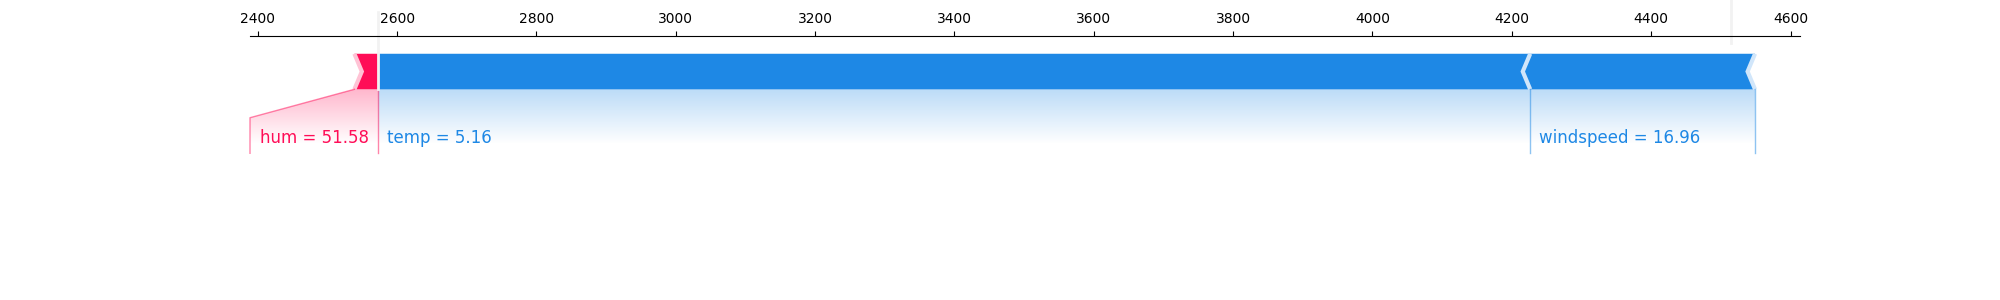
\includegraphics[width=\columnwidth]{figure_man/exSHAP.png}
%\end{figure}
%\end{frame}

\begin{frame}{Kernel SHAP - In 5 Steps}

\textbf{Definition:} A kernel-based, model-agnostic method to compute Shapley values via local surrogate models (e.g. linear model)\\
\vspace{1cm}
\begin{enumerate}
    \item Sample coalition vectors  \(\zv'\!\in\!\{0,1\}^p\)
    %\begin{onlyenv}<1>
   % $$z_{k}^{\prime} \in\{0,1\}^{M}, \quad k \in\{1, \ldots, K\}$$
    %\end{onlyenv}
    
    \item Map coalition vectors to original feature space and predict
    %Transfer coalitions into feature space \& get predictions by applying ML model
    
 %   \begin{onlyenv}<2>
  %  $$\hat{f}: \hat{f}\left(h_{x}\left(z_{k}^{\prime}\right)\right)$$
   % \end{onlyenv}
    
    \item Compute kernel weights for surrogate model
 %   \begin{onlyenv}<3>
 %   $$\pi_{x}\left(z^{\prime}\right)=\frac{(M-1)}{\left(\begin{array}{c} M \\\left|z^{\prime}\right|\end{array}\right)\left|z^{\prime}\right|\left(M-\left|z^{\prime}\right|\right)}$$
 %   \end{onlyenv}
    
    \item Fit a weighted linear model 
  %  \begin{onlyenv}<4>
  %  $$L\left(\hat{f}, g, \pi_{x}\right)=\sum_{z^{\prime} \in Z}\left[\hat{f}\left(h_{x}\left(z^{\prime}\right)\right)-g\left(z^{\prime}\right)\right]^{2} \pi_{x}\left(z^{\prime}\right)$$
  %  \end{onlyenv}

    \item Return Shapley values
%    \begin{onlyenv}<5>
%    $$(\phi_1, \ldots, \phi_M)$$
%    \end{onlyenv}
    
    
\end{enumerate}

\end{frame}



% \begin{frame}{Kernel SHAP in 5 Steps}

% \textbf{Goal:} Estimate Shapley values for a fixed instance \(\xv\) without model restrictions.

% \medskip
% \begin{enumerate}
%   \item \textbf{Sample coalitions}  
%         Draw \(K\) binary masks  
%         \(\zv'^{(k)}\!\in\!\{0,1\}^p\) (\(k=1,\dots,K\)); each mask marks a subset of “known” features.

%   \item \textbf{Create coalition inputs \& predict}  
%         Build \(\tilde{\xv}^{(k)}\) by  
%         \(\tilde{x}^{(k)}_j = x_j\) if \(z'^{(k)}_j=1\); otherwise impute.  
%         Evaluate the model: \(y^{(k)} = \fh\!\bigl(\tilde{\xv}^{(k)}\bigr)\).

%   \item \textbf{Assign kernel weights}  
%         \[
%           \pi_x(\zv') = \frac{p-1}{\binom{p}{|\zv'|}\,|\zv'|\,(p-|\zv'|)}
%         \]

%   \item \textbf{Fit weighted surrogate}  
%         Weighted least squares for  
%         \(g(\zv') = \phi_0 + \sum_{j=1}^p \phi_j z'_j\):
%         \[
%           \min_{\phi}\sum_{k=1}^K \bigl[y^{(k)} - g(\zv'^{(k)})\bigr]^2\,\pi_x(\zv'^{(k)})
%         \]

%   \item \textbf{Return Shapley estimates}  
%         Coefficients \(\phi_j(\xv)\) (and \(\phi_0\)) are the Kernel-SHAP attributions.
% \end{enumerate}

% \end{frame}


\begin{frame}{Kernel SHAP - In 5 Steps}


\textbf{Step 1: Sample coalition vectors}
\begin{itemize}
    \item Sample K coalitions from the simplified (binary) feature space
    $$\mathbf{z}^{\prime (k)} \in\{0,1\}^{p}, \quad k \in\{1, \ldots, K\}$$
    \item \( \mathbf{z}^{\prime (k)} \in \{0,1\}^p \) indicates which features are present in  \( k \)-th coalition
  \item To evaluate the model on each coal., we must map \( \mathbf{z}^{\prime (k)} \) to original space %a full feature vector in the 
  
    \item Example ($\xv = (51.6, 5.1, 17.0)$) $\Rightarrow$ $2^p = 2^3 = 8$ coals (without sampling)
    %For our simple example, we have in total $2^p = 2^3 = 8$ coalitions (without sampling)
\end{itemize}


\begin{tikzpicture}
\fontsize{8}{12}

\node (tab1) {%
\begin{tabular}{l |ccc}
  \( \mathbf{z}^{(k)} \) & hum & temp & ws \\
  \hline
  \( \mathbf{z}^{(1)} \) & ? & ? & ? \\
  \( \mathbf{z}^{(2)} \) & 51.6 & ? & ? \\
  \( \mathbf{z}^{(3)} \) & ? & 5.1 & ? \\
  \( \mathbf{z}^{(4)} \) & ? & ? & 17.0 \\
  \( \mathbf{z}^{(5)} \) & 51.6 & 5.1 & ? \\
  \( \mathbf{z}^{(6)} \) & ? & 5.1 & 17.0 \\
  \( \mathbf{z}^{(7)} \) & 51.6 & ? & 17.0 \\
  \( \mathbf{z}^{(8)} \) & 51.6 & 5.1 & 17.0 \\
\end{tabular}};

\node [left=of tab1] (tab2) {%
  \begin{tabular}{l |c|ccc}
  Coalition & \( \mathbf{z}^{\prime(k)} \) & hum & temp & ws \\
  \hline
  \( \varnothing \) & \( \mathbf{z}^{\prime(1)} \) & 0 & 0 & 0 \\
  hum & \( \mathbf{z}^{\prime(2)} \) & 1 & 0 & 0 \\
  temp & \( \mathbf{z}^{\prime(3)} \) & 0 & 1 & 0 \\
  ws & \( \mathbf{z}^{\prime(4)} \) & 0 & 0 & 1 \\
  hum, temp & \( \mathbf{z}^{\prime(5)} \) & 1 & 1 & 0 \\
  temp, ws & \( \mathbf{z}^{\prime(6)} \) & 0 & 1 & 1 \\
  hum, ws & \( \mathbf{z}^{\prime(7)} \) & 1 & 0 & 1 \\
  hum, temp, ws & \( \mathbf{z}^{\prime(8)} \) & 1 & 1 & 1 \\
  \end{tabular}};

\draw[->] (tab2.north) to[out=10,in=170] node[below]{Map to original feature space} (tab1.north);
\end{tikzpicture}


\end{frame}




\begin{frame}{Kernel SHAP – In 5 Steps}

\textbf{Step 2: Map coalition vectors to original feature space and predict}

\begin{itemize}
  \item Define mapping \( h_{\xv, \xv'} : \{0,1\}^p \rightarrow \mathbb{R}^p \):
  $
  \left(h_{\xv, \xv'}(\mathbf{z}^{\prime})\right)_j =
  \begin{cases}
    x_j & \text{if } z_j^{\prime} = 1 \\
    x_j^\prime & \text{if } z_j^{\prime} = 0
  \end{cases}
  $
  \item Construct $\zv = h_{\xv, \xv'}(\mathbf{z}')$ where present features take their values from \( \xv \) and absent features are imputed with values from a \textcolor{orange}{random background sample \( \xv' = (64.3, 28.0, 14.5)\)}
  %\item Repeat with multiple background samples to approximate marginal/conditional expectations over the absent features (example below without repetitions)
  \item Evaluate the model on each constructed vector: $\hat{f} = \hat{f}(h_{\xv, \xv'}(\mathbf{z}^{\prime(k)}))$
\end{itemize}

\medskip

\begin{tikzpicture}
\fontsize{8}{12}

\node (tab1) {%
  \begin{tabular}{l |ccc | c}
  \( \mathbf{z}^{(k)} \) & hum & temp & ws & \( \hat{f}(h_{\xv}(\mathbf{z}^{\prime(k)})) \) \\
  \hline
  \( \mathbf{z}^{(1)} \) & \textcolor{orange}{64.3} & \textcolor{orange}{28.0} & \textcolor{orange}{14.5} & 6211 \\
  \( \mathbf{z}^{(2)} \) & 51.6 & \textcolor{orange}{28.0} & \textcolor{orange}{14.5} & 5586 \\
  \( \mathbf{z}^{(3)} \) & \textcolor{orange}{64.3} & 5.1 & \textcolor{orange}{14.5} & 3295 \\
  \( \mathbf{z}^{(4)} \) & \textcolor{orange}{64.3} & \textcolor{orange}{28.0} & 17.0 & 5762 \\
  \( \mathbf{z}^{(5)} \) & 51.6 & 5.1 & \textcolor{orange}{14.5} & 2616 \\
  \( \mathbf{z}^{(6)} \) & \textcolor{orange}{64.3} & 5.1 & 17.0 & 2900 \\
  \( \mathbf{z}^{(7)} \) & 51.6 & \textcolor{orange}{28.0} & 17.0 & 5411 \\
  \( \mathbf{z}^{(8)} \) & 51.6 & 5.1 & 17.0 & 2573 \\
  \end{tabular}};

\node [left=of tab1] (tab2) {%
  \begin{tabular}{l |c|ccc}
  Coalition & \( \mathbf{z}^{\prime(k)} \) & hum & temp & ws \\
  \hline
  \( \varnothing \) & \( \mathbf{z}^{\prime(1)} \) & 0 & 0 & 0 \\
  hum & \( \mathbf{z}^{\prime(2)} \) & 1 & 0 & 0 \\
  temp & \( \mathbf{z}^{\prime(3)} \) & 0 & 1 & 0 \\
  ws & \( \mathbf{z}^{\prime(4)} \) & 0 & 0 & 1 \\
  hum, temp & \( \mathbf{z}^{\prime(5)} \) & 1 & 1 & 0 \\
  temp, ws & \( \mathbf{z}^{\prime(6)} \) & 0 & 1 & 1 \\
  hum, ws & \( \mathbf{z}^{\prime(7)} \) & 1 & 0 & 1 \\
  hum, temp, ws & \( \mathbf{z}^{\prime(8)} \) & 1 & 1 & 1 \\
  \end{tabular}};

\draw[->] (tab2.north) to[out=10,in=170] node[below]{\( h_{\xv, \xv'}(\mathbf{z}^{\prime(k)}) \)} (tab1.north);
\end{tikzpicture}

\end{frame}


\begin{frame}{Kernel SHAP – In 5 Steps}

\textbf{Step 2: Map coalition vectors to original feature space and predict}

\medskip

\textbf{Fix} \(\mathbf{z}'=(1,0,0)\); draw multiple \textcolor{orange}{background samples $\xv'^{(1)}, \dots, \xv'^{(B)}$}\\
\(\;\Rightarrow\) keep \textbf{hum}, replace \textbf{temp} and \textbf{ws} by draws from the background data.

\begin{table}\centering\small
\begin{tabular}{c|ccc|c}
Sample \(b\) & hum (from \(\xv\)) & temp (from $\xv'^{(b)}$) & ws (from $\xv'^{(b)}$)  & \(\hat{f}(h_{\xv, \xv'^{(b)}}(\mathbf{z}'))\) \\
\hline
1 & 51.6 & \textcolor{orange}{28.0} & \textcolor{orange}{14.5} & 4635 \\
2 & 51.6 & \textcolor{orange}{5.1} & \textcolor{orange}{14.5} & 3295 \\
3 & 51.6 & \textcolor{orange}{28.0} & \textcolor{orange}{17.0} & 5586 \\
$\vdots$ & \multicolumn{3}{c}{$\cdots$} & $\cdots$ \\
\end{tabular}
\end{table}

% \[
% \textstyle
% \overbrace{\frac{1}{B}\sum_{b=1}^{B}\hat{f}(h_{\xv, \xv'^{(b)}}(\mathbf{z}'))}^{\text{Monte-Carlo average}}
% \;\;\longrightarrow\;\;
% \mathbb{E}_{\mathbf{X}_{-S}}\bigl[f(\mathbf{x}_S,\mathbf{X}_{-S})\bigr]
% \]

\begin{itemize}
  \item Typically, many background samples $\xv'^{(1)}, \dots, \xv'^{(B)}$ are used to approximate the marginal expectation required for KernelSHAP via Monte-Carlo average:
  $$ \textstyle \mathbb{E}_{\mathbf{X}_{-S}}\bigl[f(\mathbf{x}_S,\mathbf{X}_{-S})\bigr] \approx
\frac{1}{B}\sum_{b=1}^{B}\hat{f}(h_{\xv, \xv'^{(b)}}(\mathbf{z}'))$$
\item Background samples \( \xv'^{(b)} \) are drawn from:
\begin{itemize}
  \item Conditional distribution \( \xv'^{(b)} \sim P_{\mathbf{X} \mid \mathbf{X}_S = \mathbf{x}_S} \) $\leadsto$ \textbf{Observational SHAP} 
  \item Marginal distribution \( \xv'^{(b)} \sim P_{\mathbf{X}} \) $\leadsto$  \textbf{Interventional SHAP}
\end{itemize}

\item The same procedure applies to every other coalition vector \(\mathbf{z}'^{(k)}\).
\end{itemize}

\end{frame}












% \begin{frame}{Kernel SHAP - In 5 Steps}


% \textbf{Step 2: Map coalition vectors to original feature space and predict}
% \begin{itemize}
%    % \item $$\hat{f}: \hat{f}\left(h_{x}\left(z_{k}^{\prime}\right)\right)$$
%    \item $\mathbf{z}^{\prime (k)}$ is 1 if features are are part of the $k$-th coalition, 0 if they are absent
%    \item To calculate predictions for these coalitions, we need to define a function which maps the binary feature space back to the original feature space
% \end{itemize}


% \begin{tikzpicture}
% \centering

% \fontsize{8}{12}

% \node (tab1) {%
%        \begin{tabular}{l |cccc}
%   $\xv^{coalition}$ &  hum & temp & ws \\
%   \hline 
%   $\xv^{\{\varnothing\}}$ & $\varnothing$ & $\varnothing$ &$\varnothing$  \\
%    $\xv^{\{hum\}}$ & 51.6 & $\varnothing$ & $\varnothing$  \\
%     $\xv^{\{temp\}}$ & $\varnothing$ & 5.1 & $\varnothing$  \\
%      $\xv^{\{ws\}}$ & $\varnothing$ & $\varnothing$ & 17.0  \\
%      $\xv^{\{hum, temp\}}$ & 51.6 & 5.1 & $\varnothing$  \\
%      $\xv^{\{temp, ws\}}$ &$\varnothing$ & 5.1 & 17.0  \\
%      $\xv^{\{hum, ws\}}$ & 51.6 & $\varnothing$ & 17.0  \\
%   $\xv^{\{hum, temp, ws\}}$ &51.6 & 5.1 & 17.0   \\
  
 
%   \end{tabular}};

% \node [left=of tab1] (tab2) {%
%      \begin{tabular}{l |c|ccc}
%   Coalition & $\mathbf{z}^{\prime (k)}$ &  hum & temp & ws \\
%   \hline 
%   $\varnothing$ & $\mathbf{z}^{\prime (1)}$ & 0 & 0 & 0  \\
%   hum & $\mathbf{z}^{\prime (2)}$ & 1 & 0 & 0  \\
%   temp &  $\mathbf{z}^{\prime (3)}$ & 0 & 1 & 0  \\
%   ws &   $\mathbf{z}^{\prime (4)}$ & 0 & 0 & 1  \\
%   hum, temp & $\mathbf{z}^{\prime (5)}$ & 1 & 1 & 0  \\
%   temp, ws & $\mathbf{z}^{\prime (6)}$ & 0 & 1 & 1  \\
%   hum, ws &   $\mathbf{z}^{\prime (7)}$ & 1 & 0 & 1  \\
%   hum, temp, ws & $\mathbf{z}^{\prime (8)}$ & 1 & 1 & 1  \\
   
 
%   \end{tabular}};
% \draw[->]
% (tab2.north) to[out=10,in=170] node[below]{} (tab1.north) ;
% \end{tikzpicture}

% \end{frame}


% \begin{frame}{Kernel SHAP - In 5 Steps}


% \textbf{Step 2: Map coalition vectors to original feature space and predict}
% \begin{itemize}
%    % \item $$\hat{f}: \hat{f}\left(h_{x}\left(z_{k}^{\prime}\right)\right)$$
%     \item Define 
% $h_x\left(\mathbf{z}^{\prime (k)}\right)=\mathbf{z}^{(k)} \text { where } h_x:\{0,1\}^{p} \rightarrow \R^{p}$
%  maps 1’s to feature values of observation $\xv$ for features part of the $k$-th coalition and 0's to feature values of a \color{orange}{randomly sampled observation} \color{black}for features absent in the $k$-th coalition
%   % \item Absent feature values are replaced by feature values of a \color{orange}{random observation} \color{black} of the dataset (permuted) $\leadsto$ permute feature values several times
%   (feature values are permuted multiple times) 
%    \item Predict with ML model on this dataset $\hat{f}: \hat{f}\left(h_{x}\left(\mathbf{z}^{\prime (k)}\right)\right)$
% \end{itemize}


% \begin{tikzpicture}
% \centering

% \fontsize{7}{12}

% \node (tab1) {%
%        \begin{tabular}{l |ccc | c}
%   $\mathbf{z}^{(k)}$ &  hum & temp & ws & $\hat{f}\left(h_{x}\left(\mathbf{z}^{\prime (k)}\right)\right)$\\
%   \hline 
%   $\mathbf{z}^{(1)}$ & \color{orange}{64.3} & \color{orange}{28.0} & \color{orange}{14.5} & 6211 \\
%    $\mathbf{z}^{(2)}$ & 51.6 & \color{orange}{28.0} & \color{orange}{14.5} & 5586  \\
%     $\mathbf{z}^{(3)}$ & \color{orange}{64.3} & 5.1 & \color{orange}{14.5}  & 3295\\
%      $\mathbf{z}^{(4)}$ & \color{orange}{64.3} & \color{orange}{28.0} & 17.0 &5762 \\
%      $\mathbf{z}^{(5)}$ & 51.6 & 5.1 & \color{orange}{14.5}  & 2616\\
%      $\mathbf{z}^{(6)}$ &\color{orange}{64.3} & 5.1 & 17.0  & 2900\\
%      $\mathbf{z}^{(7)}$ & 51.6 & \color{orange}{28.0} & 17.0 & 5411 \\
%   $\mathbf{z}^{(8)}$ &51.6 & 5.1 & 17.0 & 2573  \\
  
 
%   \end{tabular}};

% \node [left=of tab1] (tab2) {%
%      \begin{tabular}{l |c|ccc}
%   Coalition & $\mathbf{z}^{\prime (k)}$ &  hum & temp & ws \\
%   \hline 
%   $\varnothing$ & $\mathbf{z}^{\prime (1)}$ & 0 & 0 & 0  \\
%   hum & $\mathbf{z}^{\prime (2)}$ & 1 & 0 & 0  \\
%   temp &  $\mathbf{z}^{\prime (3)}$ & 0 & 1 & 0  \\
%   ws &   $\mathbf{z}^{\prime (4)}$ & 0 & 0 & 1  \\
%   hum, temp & $\mathbf{z}^{\prime (5)}$ & 1 & 1 & 0  \\
%   temp, ws & $\mathbf{z}^{\prime (6)}$ & 0 & 1 & 1  \\
%   hum, ws &   $\mathbf{z}^{\prime (7)}$ & 1 & 0 & 1  \\
%   hum, temp, ws & $\mathbf{z}^{\prime (8)}$ & 1 & 1 & 1  \\
  
%   \end{tabular}};
% \draw[->]
% (tab2.north) to[out=10,in=170] node[below]{$h_x(\mathbf{z}^{\prime (k)})$} (tab1.north) ;
% \end{tikzpicture}

% \end{frame}

\begin{frame}{Kernel shap - in 5 steps}
\textbf{Step 3: Compute kernel weights for surrogate model}\\\medskip
%\textbf{Intuition}: We learn most about individual features if we can study their effects in isolation or at maximal interaction:
%Small coalitions (few 1’s) and large coalitions (i.e. many 1’s) get the largest weights\\NB: the figure is independent from the running example

\begin{onlyenv}<1>
\textbf{Intuition:}  
We learn most about a feature’s effect when (recall multinomial coefficient in Shapley value's set definition):
\begin{itemize}
  \item it appears \textbf{in isolation} (small coalition), or
  \item in \textbf{near-complete context} (large coalition).
\end{itemize}
\(\Rightarrow\) SHAP assigns highest weights to very small and very large coalitions.

\medskip
\textbf{Note:} The figure below is illustrative and not tied to the running example.

\begin{figure}
    \centering
    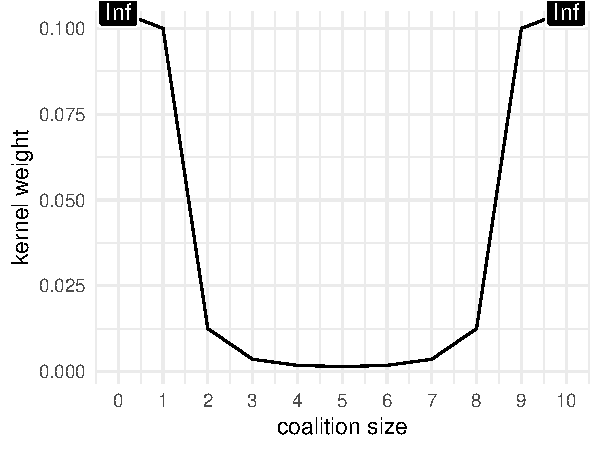
\includegraphics[width=0.5\columnwidth]{figure_man/kernel-weights.pdf}
    %\caption{Examplary dependence between kernel weights and coalition size for a data set p = 10 features}   
\end{figure}
\end{onlyenv}


\begin{onlyenv}<2>
\vspace{1cm}
\begin{exampleblock}{}
\[
\tikzmark{pi}\pi_{x}\left(\mathbf{z}^{\prime (k)}\right)=\frac{(
\tikzmark{M}p-1)}{\left(\begin{array}{c} p \\\left|\mathbf{z}^{\prime (k)}\right|\end{array}\right)\left|
\tikzmark{z}\mathbf{z}^{\prime (k)}\right|\left(p-\left|\mathbf{z}^{\prime (k)}\right|\right)}
\]
\begin{tikzpicture}[
  remember picture,
  overlay,
  expl/.style={draw=blue,fill=white,rounded corners,text width=4cm},
  arrow/.style={blue,ultra thick,->,>=latex}
]
\node[expl] 
  (piex) 
  at (2,2.5cm)
  {$\pi_x(\mathbf{z}^{\prime (k)})$: kernel weight for coalition $\mathbf{z}^{\prime (k)}$};
\node[expl] 
  (Mex) 
  at (8,3cm)
  {$p$: Number of features in $\xv$};
\node[expl] 
  (zex) 
  at (6,-1cm)
  {$\mid \mathbf{z}^{\prime (k)}\mid$: coalition size / sum of 1s in $\mathbf{z}^{\prime (k)}$};
\draw[arrow]
  (piex.south) to[out=270,in=135] ([xshift= 0.5ex, yshift=2ex]{pic cs:pi}); 
\draw[arrow]
  (Mex.south) to[out=270,in=90] ([xshift= 0.5ex, yshift=2ex]{pic cs:M}); 
\draw[arrow]
  (zex.north) to[out=90,in=250] ([xshift= 0.5ex, yshift=-1ex]{pic cs:z}); 
\end{tikzpicture}
\end{exampleblock}

\vspace{50pt}

\textbf{Note:} Weights differ from multinomial coefficient in the Shapley value set-definiton but are constructed to yield the same Shapley values via weighted linear regression.
%While this expression does not directly match the multinomial coefficient of Shapley value set definition, it is derived to produce the same weighted average over marginal contributions when using these weights in a weighted linear regression. 
\furtherreading{SEESHAP2017}
\end{onlyenv}


% \begin{onlyenv}<3>

% $$\pi_{x}\left(z^{\prime}\right)=\frac{(M-1)}{\left(\begin{array}{c} M \\\left|z^{\prime}\right|\end{array}\right)\left|z^{\prime}\right|\left(M-\left|z^{\prime}\right|\right)}$$

% \begin{itemize}
%     \item If a coalition consists of a single feature, we can learn about this feature’s isolated main effect on the prediction
%     \item If a coalition consists of all but one feature, we can learn about this feature’s total effect (main effect plus feature interactions)
%     \item If a coalition consists of half the features, we learn little about an individual feature’s contribution, as there are many possible coalitions with half of the features
% \end{itemize}
% \end{onlyenv}

% \begin{onlyenv}<4>
% \vspace{1cm}
% \textbf{Limited Budget $K$}: Can we be a bit smarter about the sampling of coalitions, than just randomly drawing?
% \begin{itemize}
%     \item The smallest and largest coalitions take up most of the weight\\ We get better Shapley value estimates by using some of the sampling budget K to include these high-weight coalitions
%     \item We start with all possible coalitions with 1 and M-1 features, which makes 2 times M coalitions in total\\ When we have enough budget left (current budget is K - 2M), we can include coalitions with 2 features and with M-2 features and so on.
%     \item From the remaining coalition sizes, we sample with readjusted weights
% \end{itemize}
% \end{onlyenv}
  
\end{frame}


\begin{frame}{Kernel shap - in 5 steps}
\textbf{Step 3: Compute kernel weights for surrogate model}\\\medskip

\only<1>{
%\textbf{Purpose}: to include this knowledge in the local surrogate model (linear regression), we calculate weights for each coalition which are the observations of the linear regression
\textbf{Purpose:} Assign observation weights $\pi_{x}\left(\mathbf{z}^{\prime}\right)$ to each coalition vector $\zv'$ when solving the local surrogate (weighted linear regression), e.g.:
%Assign weights to coalition vectors when fitting the local surrogate (linear regression) to account for their "importance"
$$\pi_{x}\left(\mathbf{z}^{\prime}\right)=\frac{(p-1)}{\left(\begin{array}{c} p \\|\mathbf{z}^{\prime}|\end{array}\right)|\mathbf{z}^{\prime}|(p-|\mathbf{z}^{\prime}|)} \leadsto \pi_x\left(\mathbf{z}^{\prime} = (1,0,0)\right)=\frac{(3-1)}{\left(\begin{array}{c} 3 \\1\end{array}\right)1\left(3-1\right)} = \frac{1}{3}$$
}


\only<2>{
\begin{itemize}
    \item For $p>3$ features, the finite weights are all 0.33 as every shown coalition has the same size ($|S|=1$ and $|-S|=2$ and vice versa for $p=3$).
    \item In general (when $p>3$), weights vary with coalition size.
    \item Empty and full coalitions receive weight $\infty$ (division-by-zero term)\\
    $\leadsto$ These coalition vectors are not used as obs. for the linear regression\\
    $\leadsto$ Instead constraints are used to ensure \emph{local accuracy} and \emph{missingness}
\end{itemize}
% $\leadsto$ all the finite weights being equal to the same value (0.33) is the result of coalition size being equal to 3. In general the weight distribution is not uniform. 
% \\$\leadsto$ weights for empty and full set are infinity (since they result in division by 0 when calculating $\pi_{x}\left(\mathbf{z}^{\prime}\right)$) and not used as observations for the linear regression\\ $\leadsto$ instead constraints are used such that properties (local accuracy and missingness) are satisfied
}

\begin{table}[]
    \centering
        \begin{tabular}{l |c|ccc|c}
 Coalition & $\mathbf{z}^{\prime (k)}$ &  hum & temp & ws & weight $\pi_{x}\left(\mathbf{z}^{\prime}\right)$\\
  \hline 
  $\varnothing$ & $\mathbf{z}^{\prime (1)}$ & 0 & 0 & 0 & $\infty$ \\
  hum & $\mathbf{z}^{\prime (2)}$ & 1 & 0 & 0 & 0.33 \\
  temp &  $\mathbf{z}^{\prime (3)}$ & 0 & 1 & 0 & 0.33 \\
  ws &   $\mathbf{z}^{\prime (4)}$ & 0 & 0 & 1 & 0.33  \\
  hum, temp & $\mathbf{z}^{\prime (5)}$ & 1 & 1 & 0 & 0.33 \\
  temp, ws & $\mathbf{z}^{\prime (6)}$ & 0 & 1 & 1 & 0.33 \\
  hum, ws &   $\mathbf{z}^{\prime (7)}$ & 1 & 0 & 1 & 0.33 \\
  hum, temp, ws & $\mathbf{z}^{\prime (8)}$ & 1 & 1 & 1 & $\infty$ \\
  
 
  \end{tabular}
\end{table}
% \medskip

  
\end{frame}

%\begin{frame}{Coalition Mapping}
%We define a coalition $z^{\prime}$, by describing a function 

%$$
%h\left(z^{\prime}\right)=z \text { where } h:\{0,1\}^{M} \rightarrow \mathbb{R}^{p}
%$$


%\begin{onlyenv}<1>
%\vspace{1cm}
%\begin{itemize}
%    \item Coalition $z^{\prime} \in \{0, 1\}^M$ is the  vector, indicating if feature $j$ contributes to the prediction 
%    \item $h(\cdot)$ represent a function that maps 1’s to the corresponding value from the observation x that we want to explain: $h(\cdot)$ connects our coalition vector to the underlying data 
%\end{itemize}
%\end{onlyenv}

%\begin{onlyenv}<2->
%\begin{tikzpicture}
%\centering

%\node<2> (tab1) {%
%  \begin{tabular}{l |cccc}
%  observation & temp & hum & ws & yr\\
%  \hline 
%  $x_{ex}$ & 24.7 & 58.5 & 13.96 & 2011\\
 % \\
 % \\
  %\end{tabular}};
%\node<3-> (tab1) {%
%  \begin{tabular}{l |cccc}
%  observation & temp & hum & ws & yr\\
%  \hline 
%  $x_{ex}$ & 24.7 & 58.5 & 13.96 & 2011\\
%  $z_{temp, yr}$ & 24.7 & $\varnothing$ & $\varnothing$ & 2011\\
%  $z_{yr}$ & $\varnothing$ & $\varnothing$ & $\varnothing$ & 2011\\
%  \end{tabular}};
%\node<2> [left=of tab1] (tab2) {%
%  \begin{tabular}{l |cccc}
%  Coalition & temp & hum & ws & yr\\
%  \hline 
%  $x^{\prime}$ & 1 & 1 & 1 & 1 \\
%  \\
%  \\
%  \end{tabular}};
%\node<3-> [left=of tab1] (tab2) {%
%  \begin{tabular}{l |cccc}
%  Coalition & temp & hum & ws & yr\\
%  \hline 
%  $x^{\prime}$ & 1 & 1 & 1 & 1 \\
%  $z^{\prime}_{temp, yr}$ & 1 & 0 & 0 %& 1 \\
%  $z^{\prime}_{yr}$ & 0 & 0 & 0 & 1 %\\
%  \end{tabular}};
%\draw<2->[->]
%(tab2.north) to[out=30,in=150] node[below]{$h(\cdot)$} (tab1.north) ;
%\end{tikzpicture}
%\end{onlyenv}
%\begin{onlyenv}<3->
%\begin{itemize}
%    \item $h(\cdot)$ maps 1’s to the %corresponding value from the observation x that we want to explain
%    \item<4> it maps 0’s to the values of another observation that we sample from the data
%    \item<4>  we equate “feature value is absent” with “feature value is replaced by random feature value from data”
%\end{itemize}
%\end{onlyenv}
%\end{frame}


% \begin{frame}{Kernel shap - in 5 steps}
% \textbf{Step 4: Fit a weighted linear model}\\\medskip
% \textbf{Aim}: Estimate a weighted linear model with Shapley values being the coefficients $\phi_j$
% $$
% g\left(\mathbf{z}^{\prime (k)}\right)=
% \phi_{0}+\sum_{j=1}^{p}
%  \phi_{j} z_{j}^{\prime (k)} \only<2>{\leadsto g\left(\mathbf{z}^{\prime (k)}\right)=
% 4515 +
%  34 \cdot z_{1}^{\prime (k)} - 1654 \cdot z_{2}^{\prime (k)} - 323 \cdot z_{3}^{\prime (k)} }
% $$


% \only<1>{
% and minimize by WLS using the weights $\pi_{x}$ of step 3
%     $$L\left(\hat{f}, g, \pi_{x}\right)=\sum_{k = 1}^K\left[\hat{f}\left(h_{x}\left(\mathbf{z}^{\prime (k)}\right)\right)-g\left(\mathbf{z}^{\prime (k)}\right)\right]^{2} \pi_{x}\left(\mathbf{z}^{\prime (k)}\right)$$

% with $\phi_0 = \E(\fh)$ and $\phi_p = \fh(x) - \sum_{j=0}^{p-1} \phi_j$ we receive a $p-1$ dimensional linear regression problem
% }

% \only<2>{
% \begin{table}[]
%     \centering
%         \begin{tabular}{l |ccc|c|c}
%   $\mathbf{z}^{\prime (k)}$ &  hum & temp & ws & weight & $\fh$\\
%   \hline 
%    $\mathbf{z}^{\prime (2)}$ & 1 & 0 & 0 & 0.33 & 4635\\
%     $\mathbf{z}^{\prime (3)}$ & 0 & 1 & 0 & 0.33 & 3087\\
%      $\mathbf{z}^{\prime (4)}$ & 0 & 0 & 1 & 0.33 & 4359\\
%      $\mathbf{z}^{\prime (5)}$ & 1 & 1 & 0 & 0.33 & 3060\\
%      $\mathbf{z}^{\prime (6)}$ & 0 & 1 & 1 &0.33 & 2623\\
%      $\mathbf{z}^{\prime (7)}$ & 1 & 0 & 1 & 0.33 & 4450\\
%       \multicolumn{1}{c}{} & \multicolumn{3}{c}{\upbracefill}&\multicolumn{1}{c}{} &\multicolumn{1}{c}{\upbracefill}\\[-1ex]
%     \multicolumn{1}{c}{} & \multicolumn{3}{c}{$\scriptstyle input$}&\multicolumn{1}{c}{} &  \multicolumn{1}{c}{$\scriptstyle output$}\\
  
 
%   \end{tabular}
% \end{table}
% }


  
% \end{frame}





\begin{frame}{Kernel shap - in 5 steps}

\textbf{Step 4: Fit a weighted linear model}\\\medskip

\textbf{Goal}\\ Estimate Shapley values \( \phi_j \) as coefficents of a local, weighted linear surrogate.
\[
\textstyle g(\mathbf{z}') \;=\; \phi_0 \;+\; \sum_{j=1}^{p} \phi_j z'_j
\]

\only<1>{
\textbf{Weighted least-squares objective}

\[
\textstyle
\min_{\phi}\;
\sum_{k=1}^{K}
\pi_x(\mathbf{z}'^{(k)})
\Bigl[
  \hat{f}\bigl(h_{\xv}(\mathbf{z}'^{(k)})\bigr)
  - g(\mathbf{z}'^{(k)})
\Bigr]^2
\]
Boundary coalitions ($\zv' = \mathbf{1}$ and $\zv'=\mathbf{0}$) enforce constraints on coefficients
\[
\textstyle 
\phi_0 = \mathbb{E}[\hat{f}(\mathbf{X})],
\qquad
\sum_{j=1}^{p} \phi_j = \hat{f}(\xv)-\phi_0 .
\]
}

%\medskip
\only<2>{
\textbf{Numeric illustration (\(p=3\))}

\[
g(\mathbf{z}')
= 4515
+ 34\,z'_1
-1654\,z'_2
-323\,z'_3
\]

\begin{table}\centering\small
\begin{tabular}{c |ccc|c|c|c}
\( \mathbf{z}' \) & hum & temp & ws & weight $\pi_{x}\left(\mathbf{z}^{\prime}\right)$ & \( \hat{f}( h_{\xv}(\mathbf{z}')) \) & \( g(\mathbf{z}') \) \\
\hline
\( (1,0,0) \) & 1 & 0 & 0 & 0.33 & 4635 & 4549 \\
\( (0,1,0) \) & 0 & 1 & 0 & 0.33 & 3087 & 2861 \\
\( (0,0,1) \) & 0 & 0 & 1 & 0.33 & 4359 & 4192 \\
\( (1,1,0) \) & 1 & 1 & 0 & 0.33 & 3060 & 2895 \\
\( (0,1,1) \) & 0 & 1 & 1 & 0.33 & 2623 & 2538 \\
\( (1,0,1) \) & 1 & 0 & 1 & 0.33 & 4450 & 4226 \\
\multicolumn{1}{c}{} & \multicolumn{3}{c}{\upbracefill}
  & \multicolumn{1}{c}{} &
  \multicolumn{1}{c}{\upbracefill} \\[-1ex]
\multicolumn{1}{c}{} & \multicolumn{3}{c}{\scriptsize inputs}
  & \multicolumn{1}{c}{} &
  \multicolumn{1}{c}{\scriptsize outputs} \\
\end{tabular}
\end{table}

The inputs and outputs are used to learn the weighted lin. regression model.
}

\end{frame}


\begin{frame}{Kernel shap - in 5 steps}
\textbf{Step 5: Return SHAP values}\\\medskip
\textbf{Intuition}: Estimated Kernel SHAP values are equivalent to Shapley values 
\begin{align*}
g(\mathbf{z}^{\prime (8)}) &= \fh(h_x(\mathbf{z}^{\prime (8)}) ) = 4515 + 34 \cdot 1 - 1654 \cdot 1 - 323 \cdot 1\\&= \underbrace{\E(\fh)}_{\phi_0} + \phi_{hum} + \phi_{temp} + \phi_{ws} = \fh(\xv) = 2573
\end{align*}

\begin{figure}
    \centering
    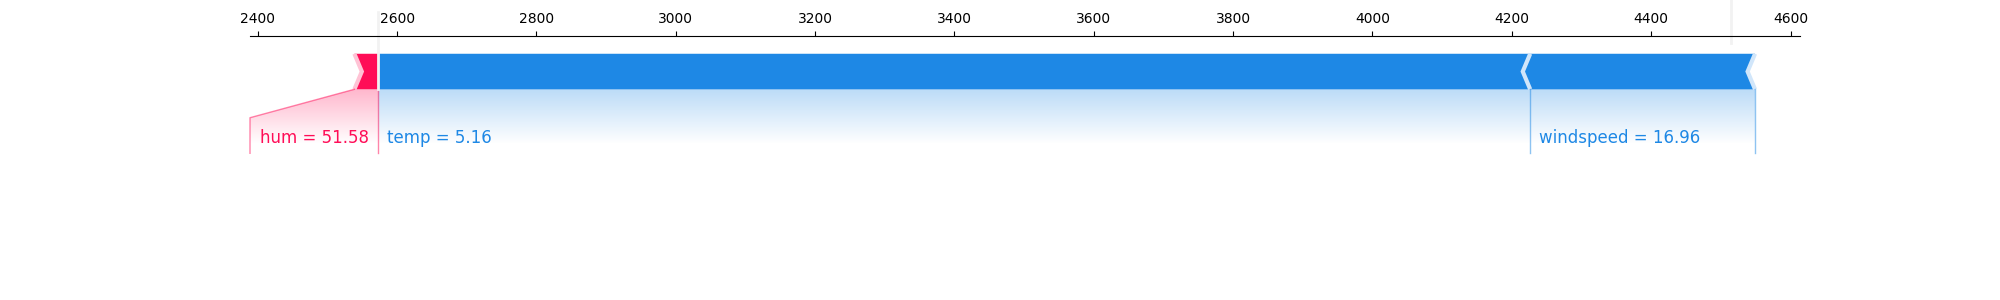
\includegraphics[width=\columnwidth]{figure_man/exSHAP.png}
    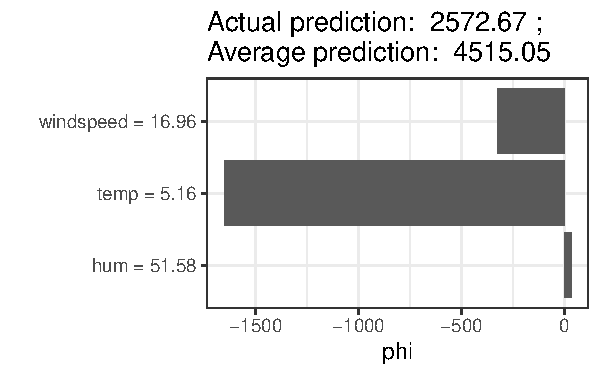
\includegraphics[trim={10 17 5 5},clip, width=0.4\linewidth]{figure/shapley2shap.pdf}
\end{figure}


\end{frame}
%\begin{frame}{Marginal Contribution}

%\begin{itemize}
%    \begin{onlyenv}<1>
%    \item Consider coalition $z^{\prime}$ as indicator function for our shapley values $\phi$
%    \end{onlyenv}
%    \begin{onlyenv}<2>
%    \item This connects the coalition vector $z^{\prime}$ to the respective marginal contribution
%    \end{onlyenv}
%    \begin{onlyenv}<3>
%    \item To estimate the marginal contribution, we can transfer the coalition to the data space by $h(z^{\prime})$
%    \end{onlyenv}
%    \begin{onlyenv}<4->
%    \item $\fh(h(z^{\prime}))$ connects the coalitions directly to the marginal distribution.
%    \end{onlyenv}
%\end{itemize}

%\vspace{1cm}

%\begin{tikzpicture}
%\centering

%\node<1-2> (tab1) {%
%  \begin{tabular}{l |cccc}
%  Coalition & temp & hum & ws & yr\\
%  \hline 
%  $x^{\prime}$ & 1 & 1 & 1 & 1 \\
%  $z^{\prime}_{temp, yr}$ & 1 & 0 & 0 & 1 \\
%  $z^{\prime}_{yr}$ & 0 & 0 & 0 & 1 \\
%  \end{tabular}};
%\node<2-> [right=of tab1] (tab2) {%
%\begin{tabular}{l | cccc}
%  & temp & hum & ws & yr\\
%  \hline 
%  $g(x^{\prime})$ & $\phi_{temp}$ + & $\phi_{hum}$ + & $\phi_{ws}$ + & $\phi_{yr}$ \\
%  $g(z^{\prime}_{temp, yr})$ & $\phi_{temp}$ + &  &  & $\phi_{yr}$\\
%   $g(z^{\prime}_{yr})$ & &  &  & $\phi_{yr}$ \\
%  \end{tabular}};
%\node<3-> [left=of tab2] (tab) {%
%  \begin{tabular}{l |cccc}
%  observation & temp & hum & ws & yr\\
%  \hline 
%  $x_{ex}$ & 24.7 & 58.5 & 13.96 & %2011\\
%  $z_{temp, yr}$ & 24.7 & %$\varnothing$ & $\varnothing$ & %2011\\
%  $z_{yr}$ & $\varnothing$ & %$\varnothing$ & $\varnothing$ & 2011\\
%  \end{tabular}};
%\draw<2>[->]
%(tab1.south) to[out=320,in=200] node[above]{$\sum \mathbb{I}_{[z^{\prime}_i == 1]} \phi_i$} (tab2.south) ;
%\draw<3->[->]
%(tab2.south) to[out=200,in=330] node[above]{$\fh(h(z^{\prime}))$} (tab1.south) ;
%\end{tikzpicture}

%\begin{onlyenv}<4>
%\begin{equation}
%\begin{array}{lllc}
  
%  g(x^{\prime}) &= \phi_{temp} + \phi_{hum} + \phi_{ws} + &\phi_{yr} &= 6825\\
%  g(z^{\prime}_{temp, yr}) &= \phi_{temp} + &\phi_{yr} &= 6134\\
%   g(z^{\prime}_{yr}) &= &\phi_{yr} &= 4325\\
%\end{array}
%\end{equation}
%\end{onlyenv}

%\begin{onlyenv}<5>
%\vspace{0.5cm}

%\textbf{Notice:}\\ We created a coalition data set $Z^{\prime}$ here by sampling multiple coalitions from observation $\xv$ that is evaluable with the prediction function $\fh$
%\end{onlyenv}

%\end{frame}



\endlecture
\end{document}
